\documentclass[conference]{IEEEtran}
\usepackage{times}

% numbers option provides compact numerical references in the text. 
\usepackage[numbers]{natbib}
\usepackage{multicol}
\usepackage[bookmarks=true]{hyperref}
\usepackage{graphicx}
\usepackage{amsmath}
\usepackage[lofdepth,lotdepth]{subfig}

\newcommand{\PAPERTITLE}{Tuning Soft Constraints in Navigation Costmaps}
\newcommand{\yhat}{\hat{y}}
\pdfinfo{
   %/Author (David V. Lu, William D. Smart)
   /Title  (\PAPERTITLE)
   /CreationDate ()
   /Subject (Robots)
   /Keywords (Robots;Overlords)
}

\begin{document}

% paper title
\title{\PAPERTITLE}

% You will get a Paper-ID when submitting a pdf file to the conference system
\author{Author Names Omitted for Anonymous Review. Paper-ID 1}

%\author{\authorblockN{David V. Lu}
%\authorblockA{Department of Computer Science \\
%Washington University in St. Louis\\
%St. Louis, MO 63108\\
%Email: davidlu@wustl.edu}
%\and
%\authorblockN{Daniel B. Allan}
%\authorblockA{Department of Physics \\
%Johns Hopkins University\\
%Balitmore, MD\\
%Email: dallan@pha.jhu.edu}
%\and
%\authorblockN{William D. Smart}
%\authorblockA{Department of Mechanical Engineering\\
%Oregon State University\\
%Corvallis, OR 97331\\
%Email: bill.smart@oregonstate.edu}}

\maketitle

\begin{abstract}
Costmaps are increasingly being used for purposes other than marking a location in a robot's environment as occupied. Researchers in Human Robot Interaction have used intermediate costmap values to help improve robot navigation in proximity to people. Costmaps with non-zero non-lethal values allow it to represent policies with soft constraints, such as not getting too close to people, or only entering a region when absolutely necessary. This can help improve the quality of interactions and the efficiency of both parties' navigation. 

While constant and Gaussian distributed additions to costmaps are already in use, there has been no general strategy for how to set up the parameters of the additions to ensure the desired behavior is achieved. In this paper, we describe how the parameters for the soft constraints can affect the robot's planned paths, and what constraints on the parameters can be introduced in order to achieve certain behaviors. 

Gaussian distributions, which are oft used to model people's personal space, have several interesting properties. In order to plan a path that is a set distance away from the obstacle, the ratio of the constant added for each cell traversed in a path to the amplitude of the Gaussian needs to be a positive number less than approximately $.57$.  There are also irregularities in the Gaussian parameter space which result in discontinuities in the resulting behavior space. Our mathematic models were check using two tests. The first actually runs a path planning algorithm on simulated costmaps. The second uses the ROS Navigation packages to plan real paths using live data and more advanced planning algorithms. Both tests confirm the properties of the soft constraints that result in the different behaviors. 

%Satisfying soft constraints like these have the capability to improve a person's comfort and safety around a robot, as well as improve the efficiency of the robot. 

\end{abstract}

\IEEEpeerreviewmaketitle
\section{Introduction}
Navigating through an environment is one of the fundamental tasks in mobile robotics. For robots with relatively reasonable dynamics and operating speeds in indoor environments, efficient collision-free navigation is practically solved. However, introducing constraints other than ``please take the shortest path without running into anything'' is still an ongoing area of research, especially when taking the social needs of humans into account. These constraints often take the form of non-lethal obstacles, or places that are undesirable to be but do not result in a collision. Modeling non-lethal obstacles in the space around a person will help robots to not invade the person's personal space. 

These representations raise the value of a set of cells in the costmap, making it less likely for the robot to travel in them. In the person-avoiding scenario, this means that the robot will respect the person's personal space more often, since the areas closest to the person will have the highest costs.

However, it is not always the case though that higher costs result in the robot not traveling through a given cell. The robot still could drive through a person's intimate social space given the right circumstances. Such a path would be inoptimal when considering the person's proxemic concerns, but it is still valid and non-lethal (i.e. does not result in a collision). Sometimes this behavior corresponds with the proxemically inoptimal path being the only path available. However, sometimes it results from improperly tuned parameters. While the previous researchers have all tuned their parameters to create working configurations, there exists no general guide for understanding the process of how the parameters change the robot behavior. Furthermore, as our exploration of this space shows, the behavior is not always readily intuitive. 

This paper aims to explore the space of these paths through non-lethal costmaps. 


\begin{figure}
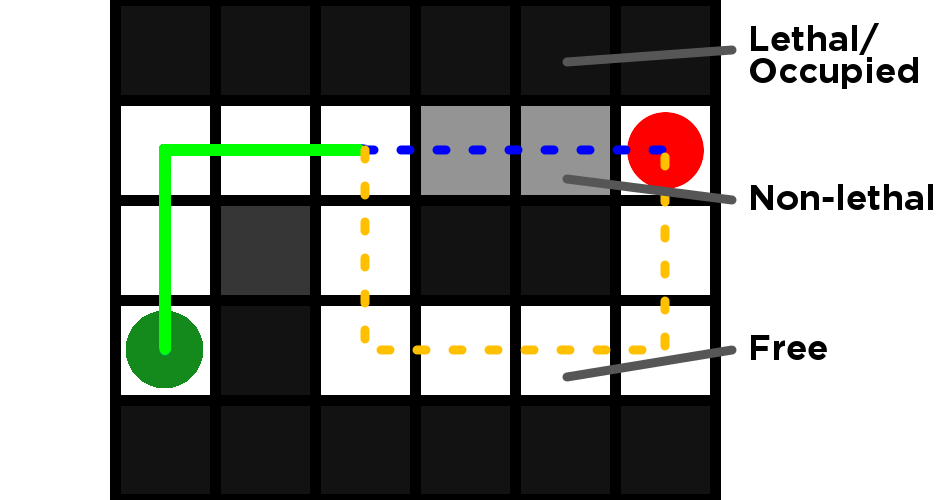
\includegraphics[width=\columnwidth]{graphix/Intro.png}
\caption{Simple Costmap with Non-lethal Obstacles -  In a costmap, the world is discretized into cells. Each cell has a value $f(x,y)$. If the value is greater than some limit $L$, they are considered ``lethal'', meaning that there is an obstacle somewhere in that cell, and entering it will result in a ``lethal'' collision. Cells with a value of zero are considered free, i.e. there is no penalty for entering the cell. Everything in between is a ``non-lethal'' obstacle, meaning there is some reason not to be in the cell, but it won't cause a collision. The robot could either continue along the blue path (the shortest path), or it could take a longer yellow path but avoid the non-lethal obstacle. Which path is optimal and which is the path less traveled depends on how the costmap \emph{and} the path planner are configured. }
\label{fig:intro}
\end{figure}

\section{Related Work}
Methods for avoiding a person while navigating in a hallway have existed for some time. Early works like \citet{yoda1997} took a single person into consideration, but assumed a static behavior. Later work by \citet{christensen2004} realized that a more complex world model was needed for such a task and integrated the distance to multiple people and conversation formations into the navigation algorithm. 
\citet{christensen2005} further explored robots navigating around people with explicit consideration of the proxemic zones found in the work of \citet{hall1969}. However, all of these approaches controlled navigation directly with a velocity controller, limiting long term planning and ways the constraints could be formulated. 

Most uses of soft constraints in costmaps have been for representing a person's personal space. \citet{dautenhahn:serveseated} %2006 sisbot 
constructed recommendations for planning motions where humans would be comfortable based on live HRI trials, taking proximity, visibility and hidden zones into consideration. These were formulated into a costmap system by \citet{sisbot2007}, creating a Gaussian based ``human aware motion planner.'' 
\citet{kirby:companion} used an algorithm that in addition to minimizing path distance and avoiding obstacles, modeled proxemics and behaviors like passing on the right into the costmap, also using Gaussians. 

Work by \citet{svenstrup2009}\cite{svenstrup2010} created even more complicated models of personal space, integrating a mixture of four different constraints modeled as Gaussians.  expanded this work to maneuver among a field of multiple people while moving toward a goal. 

Among the latest work in this field, \citet{sisbot2011} have expanded their original model to a three dimensional costmap in order to control positioning during hand off tasks, taking safety, visibility and the human's arm comfort into consideration. \citet{fraichard:anthronav} have also created a complex model that included proxemic, visibility and motion models as Gaussians, and ``interaction areas'' as constants. 

Soft constraints are occasionally used for other fields like autonomous vehicles. \citet{likhachev:costmaps} used large constant valued areas to favor driving on the right side of the road and to avoid curbs. 

Most of the obstacles added to the costmaps follow Gaussian distributions or constant values (with the minor exception of the representation of the intimate personal space in the work by \citet{fraichard:anthronav}). Little to no discussion is given about how the authors of the previous works found the parameters that worked best with their system. 

% christensen Parameters for interactions with people - robot speed, signaling distance, lateral distance







\section{Problem Statement}
%We define the problem of path planning as follows: Given a start point and an end point, find the ``best'' path between them, where the definition of ``best'' depends on a set of preferences. Traditionally, the selected path will depend on two things: the location of obstacles and the length of the path, i.e. the planned paths are generally the shortest path to the goal that avoids collisions with any other objects. Finding such a path is generally easy. However, beyond avoiding collisions and getting to the destination efficiently, there are a number of other factors that can factor into which path is considered ``best.'' 

We define the problem of path planning with non-lethal constraints as follows: find a path from a starting location to a goal while not colliding with any obstacles and maximizing the distance from the path to a set of non-lethal obstacles while minimizing the overall length of the path. The duality of maximizing the one quantity while minimizing the other results in a continuum of different paths that could be considered optimal depending on the weighting of the two sides. 

\begin{figure}
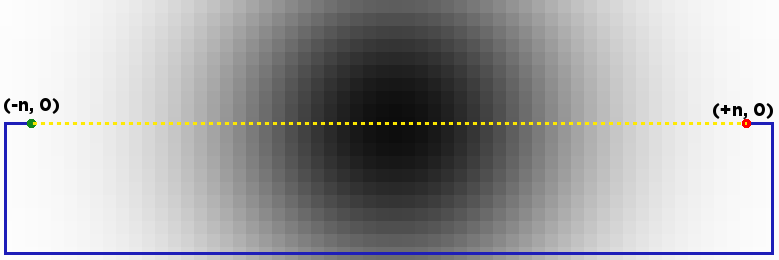
\includegraphics[width=\columnwidth]{graphix/TwoPaths.png}
\caption{Two Simple Paths - The dotted yellow path is the shortest possible path. The solid blue path is the path with the lowest possible cost (within the bounds of the costmap). The tint of each cell is proportional to its cost. The green and red dots indicate the start and goal points respectively. }
\label{fig:twopaths}
\end{figure}

%The prioritization is separated into two different subsystems. First, there is the costmap where the value of the cells is stored. If only the

If we prioritize the shortest possible path (as most planners do), we end up with the straight path seen in Figure \ref{fig:twopaths}, which does not make any attempt to avoid the obstacle. (Note that there are no lethal obstacles shown in the figure.) However, the lowest cost regions are along the border of the costmap, so if lowest cost becomes the priority, a longer more round-about path will be taken. 

A more formal statement of the problem includes the following elements. First, a grid of discretized cells lying in a two dimensional plane, denoted by $x$ and $y$. Each cell has a non-negative cost, denoted by $C(x,y)$, where all cells with $C(x,y)\ge L$ are considered to be lethal, and the rest are non-lethal.  Given starting and goal cells (from the non-lethal subset), find a path from one to the other moving through only non-lethal cells that minimizes the length and total cost. 

In the case of a 4-connected grid, one way of calculating such a path is

\[ \min_{\forall \mathrm{path} p} C(p) = \min_{\forall \mathrm{path} p} \sum\limits_{(x,y) \in p}^{} \Big[ f(x,y) + P \Big] \]

where $C(p)$ represents the combination of the path length and summation of $f(x,y)$, and $P$ is the path constant. That is to say, in addition to minimizing the total cost, we minimize the total cost plus some constant value for each cell entered. The value of $P$ is our primary means of controlling how much path length is considered vs. total cost. If $P=0$, then the long path in Figure \ref{fig:twopaths} will be planned, and if $P$ is rather large, the short straight path will be taken. 


For our initial pass analyzing these paths, we are going to assume for simplicity a 4-connected grid rather than an 8 or more connected grid, since such paths would involve scaling the costs and path constant proportionally to how long the path is in each cell. 

For purposes of this paper, let us further refine the problem to reduce the number of cases we must consider. First, let us consider paths that go from $(-n, 0)$ to $(n, 0)$. This means that the costmap will be aligned to the primary direction of travel (i.e. the shortest path passes through $2n$ cells. When these are unaligned, the paths can be substantially different in shape, and will require analysis beyond the scope of this paper. We further assume that there are no lethal cells in our costmap, since path planning algorithms already do a fine job of avoiding lethal obstacles. Ergo, for now, we can presume that any non-lethal plan is a repeated application of planning with only non-lethal obstacles. 

In the following sections, we will see how different selections for $f$ and how $f$ is parameterized can have vastly different effects on the path. 

\section{Constant Value}
Some non-lethal obstacles are defined by a flat step cost, such as the interaction areas of \citet{fraichard:anthronav} or the perimeter of the parking lot in \citet{likhachev:costmaps}. In this trivial case, the marginal cost is
\begin{equation}
   \displaystyle
   f(x, y) = \left\{
     \begin{array}{lr}
       A & : (x,y) \in Q\\
       0 & : (x,y) \notin Q
     \end{array}
   \right.
\end{equation}
Each step traversing the obstacle costs a premium $A$. 

\begin{figure}[!t]
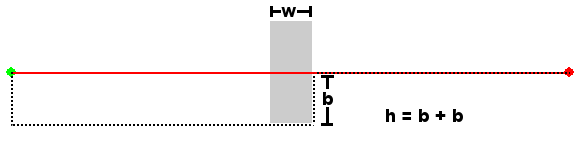
\includegraphics[width=\columnwidth]{graphix/Constant.png}
\caption{Two Paths with a Constant Non-lethal obstacle}
\label{fig:constant}
\end{figure}

We will plan a path from $(n, 0)$ to $(-n, 0)$, computing the cost by summing the baseline cost-per-step $P$ and the marginal cost-per-step $f$ over each step.

\begin{equation}
C(p) = \sum\limits_p P + f(x, y)
\end{equation}

For a rectangular step obstacle placed at the origin, there are two feasible paths as shown in Figure \ref{fig:constant}. The direct path costs
\begin{equation}
C(p_1) = 2nP + wA
\end{equation}

where $P$ is the baseline cost per step and $w$ is the width of the obstacle. The shortest path around the obstacle costs

\begin{equation}
C(p_2) = (2n + h)P.
\end{equation}

The direct path is cheaper when the aspect ratio of the obstacle  is greater than the fractional cost penalty:

\begin{equation}
\frac{h}{w} > \frac{A}{P}.
\end{equation}

This result is intuitive. If an obstacle is thin or short, walk through it.





\section{Smooth Obstacles}
The step-avoiding route shown in Figure 2 is only one example among a family of routes with equal cost. A smoothly-varying obstacle breaks this degeneracy and determines a finite number of optimal paths.

By smoothly-varying, we mean that the derivative of $f$ is defined everywhere. One such example, commonly used to model obstacles, is the Gaussian.

\begin{equation}
f(x, y) = A \exp\left(-\displaystyle\frac{x^2+y^2}{2\sigma^2}\right)
\end{equation}

The Gaussian is radially symmetric, and it decreases monotonically from its center. Both properties are sensible ones for modeling a simple obstacle.

Restricted rook-like motion in our 4-connected space, we can immediately see that all movements take the shape of a bracket: a path from $(-n,0)$ to $(-n, \yhat)$ to $(n, \yhat)$ to $(n,0)$ for some $\yhat$. (Or, equivalently, the mirror image in $y \rightarrow -y$.) If any traverse steps are taken, they should always be taken at the edge of the space, as far from the origin as possible.

\begin{figure}
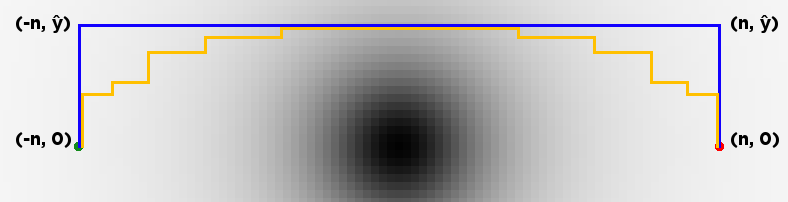
\includegraphics[width=\columnwidth]{graphix/bracket.png}
\caption{The Bracket Shape}
\label{fig:bracket}
\end{figure}
\subsection{Typical Behavior}

The previous section asserted that, whatever the model parameters, optimal paths conform to a bracket shape. One might suppose that increasing the width of the obstacle $\sigma$ or the relative cost $A/P$ causes $\yhat$ to increase commensurately, giving the obstacle a wider and wider berth. This dependence is observed for large $\yhat$, but when parameters are tuned to draw the optimal path closer to the origin, it undergoes a discontinuous jump from a finite bracket to the direct path ($\yhat=0$). As an example, consider the path in Figure \ref{fig:gaussian}. When $A/P=?/55$, a long walk around is cheap compared to treading on the origin, and the closest approach $\yhat$=16. (In this simulation, the other parameters were fixed arbitrarily at $n=?$ and $\sigma$=?.) However, when the baseline cost is dialed back such that $A/P=?/56$, the path jumps discontinuously through the origin ($\yhat=0$). Intermediate paths are not cost-effective: at a certain point, what we save by avoiding the dead center is not worth the extra steps.

\begin{figure}
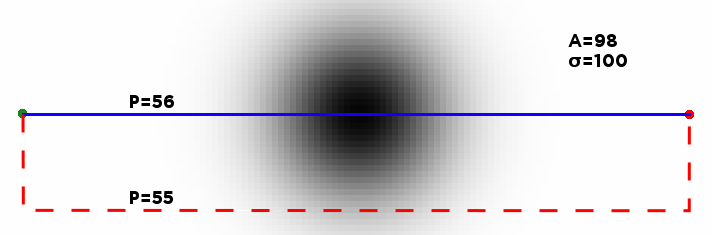
\includegraphics[width=\columnwidth]{graphix/Gaussian.png}
\caption{Gaussian Cost Function - Straight path is optimal when $P=56$, the bracket path when $P=55$. }
\label{fig:gaussian}
\end{figure}

\subsection{Mathematical Explanation}
Our goal is to show why there are certain parameters that result in one of the three behaviors discussed. 
\begin{enumerate}
\item Minimum path cost is at $\yhat=0$
\item Minimum path cost is at finite $\yhat>0$
\item Minimum path cost is infinitely far away. 
\end{enumerate}

The cost of a bracket path in terms of the model parameters and some choice of $\yhat$ is 
\begin{align*}
C(p_{\yhat}) =& C(\text{segment 1}) + C(\text{segment 2}) + C(\text{segment 3}) \\
=&\Big[\yhat P + \sum\limits_{i=0}^{\yhat-1} f(-n, i) \Big] +
         \Big[2nP + \sum\limits_{x=-n}^{n}    f(x,\yhat) \Big]\\
     &+\Big[\yhat P + \sum\limits_{i=0}^{\yhat-1} f(n, i) \Big].
\end{align*}

Now let us assume that we begin far from the obstacle, so $n \gg \sigma$; in this limit, the cost due to the obstacle on segments 1 and 3 is very small compared to the baseline cost and the cost along segment 2.
\begin{equation}
C(p_{\yhat}) \approx (2n+2\yhat)P +  \sum\limits_{x=-n}^{n} f(x,\yhat)
\end{equation}

We are only concerned with the cost of each path in relation to other paths, so we will express the cost of some $p_{\yhat}$ relative to the cost of the direct path like so. 
\begin{align*}
\Delta C(\yhat) =& C(\yhat)-C(0) \\
=& \Big[(2n+2\yhat)P +  \sum\limits_{x=-n}^{n} f(x,\yhat) \Big] \\
 & - \Big[(2n+2(0))P +  \sum\limits_{x=-n}^{n} f(x,0) \Big] \\
=& 2P\yhat + \sum\limits_{x=-n}^{n} \Big[ f(x,\yhat)-f(x,0) \Big]
\end{align*}

When $\Delta C < 0$ for some $\yhat$, the direct path is not optimal.

With a Gaussian obstacle as $f$,
\begin{equation}
\Delta C(\yhat) = 2P\yhat + \sum\limits_{x=-n}^{n} \left[A\exp\left(-\frac{x^2 + \yhat^2}{2\sigma^2}\right) - A\exp\left(-\frac{x^2}{2\sigma^2}\right) \right]
\end{equation}

We have already assumed $n \gg \sigma$, so we can approximate the sum over $x \in [-n, n]$ as the sum over all $x$, which has a simple solution. The tails of the Gaussian contribute negligibly.

\begin{equation}
\sum\limits_{x=-n}^{n} \rightarrow \text{Future Dan will sort this out.}
\end{equation}

Finally, we have a closed-form expression for the cost of bracket path $p_{\yhat}$ compared to the direct path.
\begin{equation}
\Delta C(\yhat) = 2P\yhat + A\sigma\sqrt{2\pi}\left[\exp\left(-\frac{\yhat^2}{2\sigma^2}\right) - 1\right]
\end{equation}

Now, we locate the $\yhat$ that minimize $\Delta C$.
\begin{align}
\frac{d\Delta C}{d\yhat} = 
&2P - \frac{\yhat}{\sigma}A\sqrt{2\pi} \exp\left(-\frac{\yhat^2}{2\sigma^2} \right) = 0 \\
  \frac{P}{A} =& \sqrt{\frac{\pi}{2}} \frac{\yhat}{\sigma} \exp\left(-\frac{\yhat^2}{2\sigma^2} \right)
\end{align}
\begin{figure}
\centering
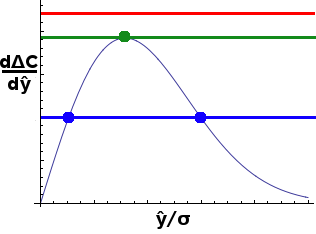
\includegraphics[width=0.4\columnwidth]{graphix/lambert.png}
\caption{Plot of $x \exp(-x^2)$, with lines marking values where the equation has no solutions (top line), one solution (middle line) or two solutions (bottom line).}
\label{fig:lambert}
\end{figure}

To find the cheapest path, we must be solve for $\yhat$ and plug it into $\Delta C(\yhat)$. The solution for $\yhat$ is related to the Lambert W-function, which is cannot be written in closed form.  Further, depending on the cost ratio $P/A$, it can admit 0, 1 or 2 solutions. This means that the Relative Cost has critical points at those solutions and the limits. From this, there are several key observations we can make. 
\begin{enumerate}
\item Two critical points are necessary for there to be a finite $\yhat>0$, as seen in Figure \ref{fig:twosolutions}. 
\item It is not sufficient to have two critical points to cause a finite $\yhat>0$, since the minimum may not have a negative value, meaning that the optimal path will be at $\yhat=0$. Similar scenario occurs when there is only one critical point as in Figure \ref{fig:inflection}. 
\item If there are no critical points as in Figures \ref{fig:zero} and \ref{fig:infinity}, then the extrema must be at the limits. If $P>0$, you end up with a positive slope like in Figure \ref{fig:zero} and the optimal minimum cost path is at $\yhat=0$. If $P=0$, then you get a negative slope and the minimum value is at $\yhat=\infty$. This follows the intuition where if $P$ is very high, then the straight path is optimal, and if $P=0$, the path length does not matter and the path can be arbitrarily far away. 
\end{enumerate}

\begin{figure}[t]
\centering
\subfloat[Two Critical Points: $\yhat>0$]{
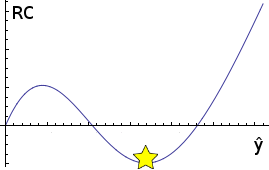
\includegraphics[width=0.4\columnwidth]{graphix/twosolutions.png}
\label{fig:twosolutions}}
\qquad
\subfloat[One Critical Point: $\yhat=0$]{
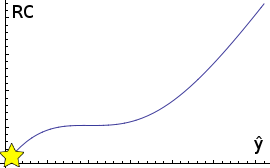
\includegraphics[width=0.4\columnwidth]{graphix/inflection.png}
\label{fig:inflection}}\\
\subfloat[No Critical Points: $\yhat=0$]{
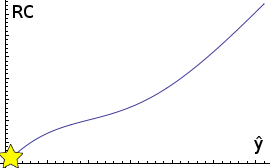
\includegraphics[width=0.4\columnwidth]{graphix/zero.png}
\label{fig:zero}}
\qquad
\subfloat[No Critical Points, $P=0$: $\yhat=\infty$]{
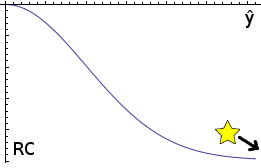
\includegraphics[width=0.4\columnwidth]{graphix/infinity.png}
\label{fig:infinity}}
\caption{Gaussian Relative Costs (y-axis) over different passing distances. Minimum cost/optimal path marked with a star. In (a), the optimum passing distance is at a finite $\yhat>0$. In (b) and (c) the optimum is at $\yhat=0$. In (d), the optimum is as far away as possible. }
\label{fig:globfig}
\end{figure}


%\section{New Cost Functions}
%\subsection{Inverse Cost Function}

%\section{Other Path Planning}
Probably going to end up removing this section, but the math in it led me to the math of the previous section. 

\subsection{One Dimensional Hazard}
Now assume that there is a hazardous area that has a relative cost proportional to the distance from the y axis, i.e. some value $f(x)$. Assuming zero cost elsewhere, the shortest path is going to be similar to the path shown in figure \ref{oneD}.
\begin{figure}
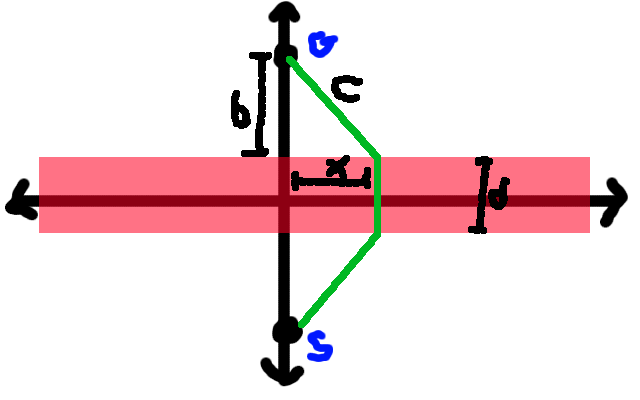
\includegraphics[width=\columnwidth]{graphix/oneD.png}
\label{oneD}
\caption{One Dimensional Setup}
\end{figure}
Let us define the path going through point $(x,0)$ to be $p(x)$. The cost of such a path will be 
\begin{align*}
C(p(x)) &= P * (2*c+d) + f(x) \\ 
 &= P * (2 * \sqrt{x^2 + b^2} + d) + f(x)
\end{align*}
If we want to force the path to cross at a certain point (call it $m$), we need to set $f(x)$ in such a way that $C(p(x))$ is a minimum. To do that we take the derivative of $C(p(x))$. 
\begin{align*}
C'(p(x)) &= f'(x) + \frac{2Px}{\sqrt{x^2+b^2}} \\
\intertext{If we set the derivative to 0}
f'(x) &= -\frac{2Px}{\sqrt{x^2+b^2}}
\intertext{Since we assert that this minimum occurs at $x=m$}
&= -\frac{2Pm}{\sqrt{m^2+b^2}}
\intertext{Integrating we get...}
f(x) &= D - \frac{2Pmx}{\sqrt{m^2+b^2}}
\end{align*}
for some constant D. 

\section{Experimental Results}
%Previously we defined good paths in terms of the actual cost of the path in relation to the costmap. However, these metrics are not necessarily the ones we ultimately want to use when we move up to an interaction mindset. 

%\subsubsection{Path Length}
%\subsubsection{Closest Approach Distance}
%\subsubsection{Average Distance to Obstacle}

If we were simply to accept the path with the lowest total cost as ``the best,'' we could now rest, assured that Dijkstra's algorithm would find the optimal path. However, in robotics, and particularly human robot interaction, there are other metrics that weigh on the value of a path. The one that is of most use to us here is the closest distance between the path and the obstacle. With the bracket shape we discussed earlier, that metric has the value of $\yhat$. There are many other metrics that we could consider, including the path length and the average distance from path to obstacle, however, those measures work proportionally to the closest distance in all of the cases considered here. A further analysis of different path metrics is considered in the Future Work section. 

Given the estimates and approximations that were needed to mathematically explain some of the properties of the Gaussian non-lethal obstacles, to fully understand their behavior, we must actually run the path planning algorithms. Costmaps were set up using the general scenario described in Section II and with the functions described below. For each set of parameters, a path was planned and the closest distance / $\yhat$ was calculated. 

For the constant non-lethal obstacle, we found that the derived paths followed the exact pattern set up by our inequality. For instance, a $5\times5$ constant valued obstacle ($w=5$) required traversing six extra cells to go around ($d=6$) and when the path constant was fifty ($P=50$), the amplitude required to force the algorithm to chose a path that went through the obstacle was $A<60$, i.e. the solution to equation (1). All amplitudes less than 60 resulted in the straight path, and all greater than 60 resulted in the path that goes around. When $A=60$, the two paths have equal cost, but only one  is returned.

\begin{figure}
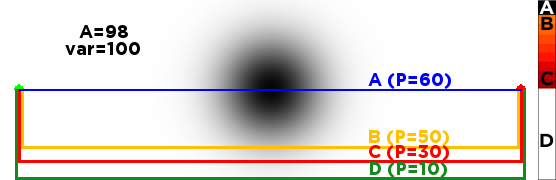
\includegraphics[width=\columnwidth]{graphix/SomePaths.png}
\caption{Paths around a Gaussian with Varying Path Constant - As $P$ decreases from (A) to (D), the path gets further and further away from the nonlethal obstacle, reflecting the length of the path becoming less important.}
\label{fig:somepaths}
\end{figure}

For the Gaussian non-lethal obstacle, the results of the simulation are a bit more complex. We know that there are certain values of parameters that result in specific behaviors, which we can see from Figure \ref{fig:colormaps}. For instance, according to equation (2), if $P/A$ is too high, there will be no solution and the optimal path will be at $\yhat=0$. We can see this in all four graphs of Figure \ref{fig:colormaps}, in that there are black areas (representing $\yhat=0$) for the large values of P and small values of A. We can also see in Figure \ref{fig:gap} that P and A have a linear relationship, which means that as long as the ratio of $P:A$ remains constant, the value of $\yhat$ will remain constant as well (given a particular variance). 

The relationship between variance and $\yhat$ is a bit more complicated, which is logical given equation (2). For any given finite positive value of $\yhat$ we can decrease the variance to get a smaller $\yhat$. This can be seen in Figure \ref{fig:gvp} for instance, where you can pick any colored point and move to a lesser variance (to the left) and get a lower $\yhat$. However, the extent to which decreasing the variance will decrease $\yhat$ depends on the other variables. 

Conversely, increasing the variance (moving to the right) can result in multiple behaviors. As expected, increasing the variance will move the closest distance as far away as possible, until it hits the border of the grid. This edge behavior can be seen in the white area on the bottom right portion of Figure \ref{fig:gvp}. At these values, the path is the maximal distance it can be away from the obstacle while still in the bounds of the grid. However, for the top portion of that figure, increasing the variance can actually \emph{decrease} the closest distance, all the way to $\yhat=0$. This corresponds with the fact that $ \sqrt{\frac{\pi}{2\sigma^2}} \yhat \exp\Big( \frac{-\yhat^2}{2\sigma^2} \Big) $ approaches 0 as $\sigma$ increases, which means that $P/A$ needs to have even smaller values to ensure a positive finite solution. 

Lastly, it is worth noting that the relationship between amplitude and path constant is a key contributor to the ease of tuning parameters. Consider Figure \ref{fig:gav} where $P=10$ and Figure \ref{fig:gav2} where $P=25$. When $P$ is relatively low, there are many valid parameter combinations to get positive $\yhat$. However, with a higher $P$, there are significantly fewer options. In some cases, it does not matter what variance you dial in, $\yhat$ will not change from being 0. 

\newcommand{\szsz}{.42}
\begin{figure}[t]
\centering
\subfloat[Amplitude vs. Path Constant]{
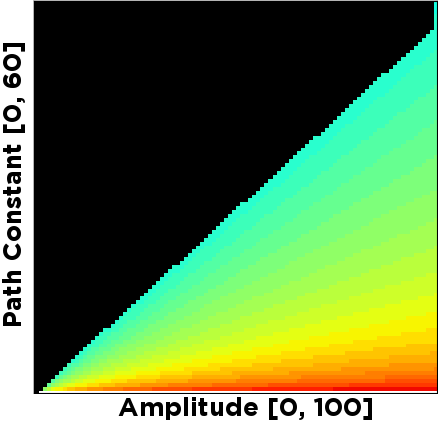
\includegraphics[width=\szsz\columnwidth]{graphix/gap.png}
\label{fig:gap}}
\qquad
\subfloat[Variance vs. Path Constant]{
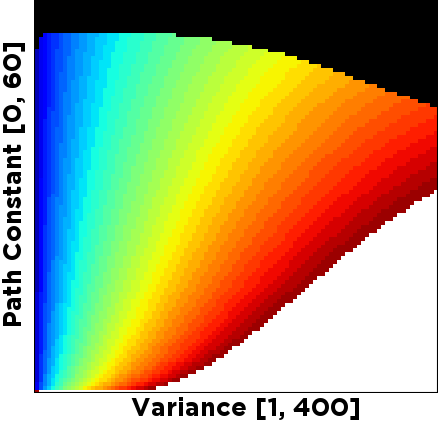
\includegraphics[width=\szsz\columnwidth]{graphix/gvp.png}
\label{fig:gvp}}\\
\subfloat[Amplitude vs. Variance \newline($P=10$)]{
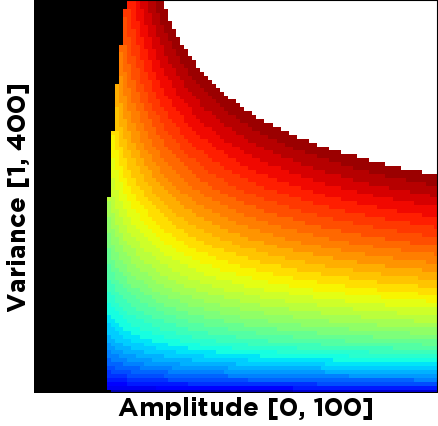
\includegraphics[width=\szsz\columnwidth]{graphix/gav.png}
\label{fig:gav}}
\qquad
\subfloat[Amplitude vs. Variance \newline($P=25$)]{
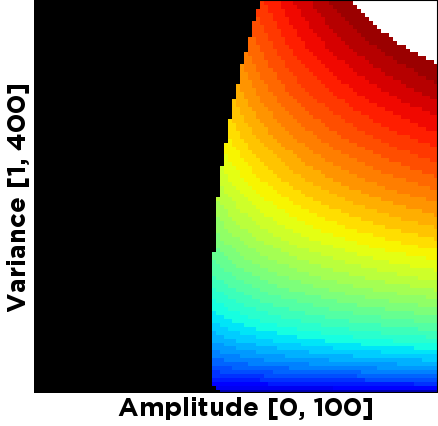
\includegraphics[width=\szsz\columnwidth]{graphix/gav2.png}
\label{fig:gav2}}
\caption{Heat Maps of $\yhat$ for different parameters for a Gaussian obstacle- The black areas mark where the path goes straight through the obstacle ($\yhat=0$), i.e. where the path constant is too high or the amplitude is too low. The white areas mark where the optimal path is as far away from the obstacle ($\yhat=\infty$), i.e. where the path traces the outer boundaries of the grid. Everything else is where $\yhat$ has a positive finite value, color coded with red paths being the longest and blue paths being the shortest.}
\label{fig:colormaps}
\end{figure}


\section{Robot Results}
Much of this work is motivated by our experiences with the ROS navigation stack \cite{marder:office}. Initially, it did not have a way to directly input non-lethal obstacles. One could only input lethal obstacles, and have a small buffer of non-lethal obstacles surround it, which made it difficult to model people's personal space. As a result, we created a branch of the navigation stack that allowed for arbitrary changes to be made to the costmap. Typical parameters for the global costmap involve a grid resolution of 5 centimeters and a planning constant of $P=50$. Amplitudes can range from $[0, 254]$ and variance was typically set between $0$ and $2$. The robot was command to move from $(-3[m], 0)$ to $(+3[m], 0)$. The costmap data is then passed into a modified wavefront planner that performs interpolated gradient descent to determine a smooth path, one not constrained by the shape of the grid. The robot used to perform the sensing of the environment was Willow Garage's PR2. For these experiments, only data from the base planar laser range finder. 

The biggest question that these experiments intended to figure out was whether the same relations between parameters that we observed in the simple 4-connected grid would hold up in this less restricted environment. As seen in Figure \ref{fig:realdata}, the same principles apply. Since costmaps and the discretized paths they produce are all approximations of the same continuous space, it is logical that the different grid connectivities would have similar results, however, it is nice to have the technical confirmation to back up the ideas. Not only is the solution more general, but it has the added benefit that the resulting smoother paths are more legible to people observing the robot. 


\newcommand{\rrrr}{.3}
\begin{figure*}[b]
\centering
\subfloat[$A=250$, $\sigma=0.15$]{
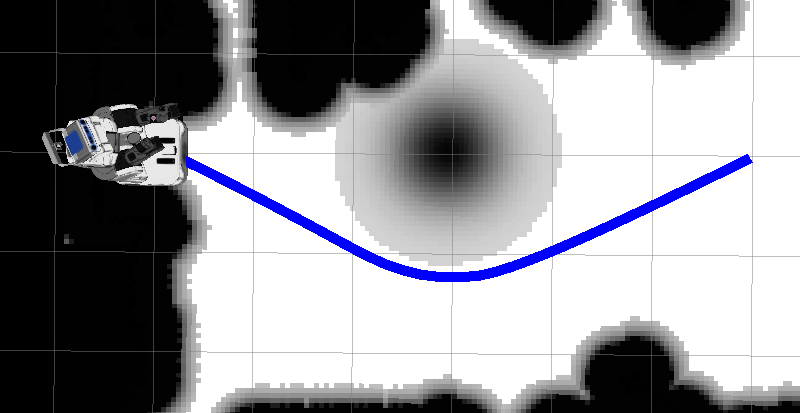
\includegraphics[width=\rrrr\textwidth]{graphix/250-p15.png}
\label{fig:d1}}
\subfloat[$A=250$, $\sigma=0.30$]{
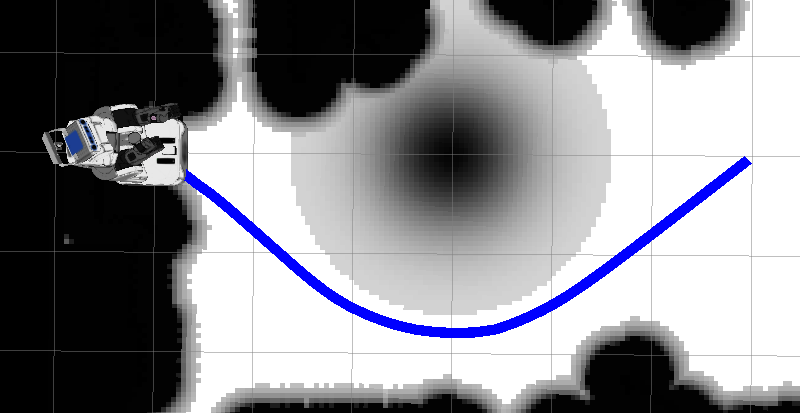
\includegraphics[width=\rrrr\textwidth]{graphix/250-p3.png}
\label{fig:d2}}
\subfloat[$A=250$, $\sigma=0.60$]{
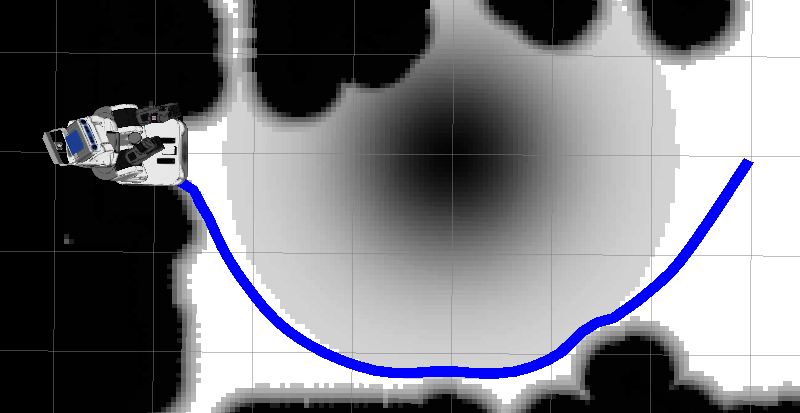
\includegraphics[width=\rrrr\textwidth]{graphix/250-p6.png}
\label{fig:d3}}\\
\subfloat[$A=250$, $\sigma=0.90$]{
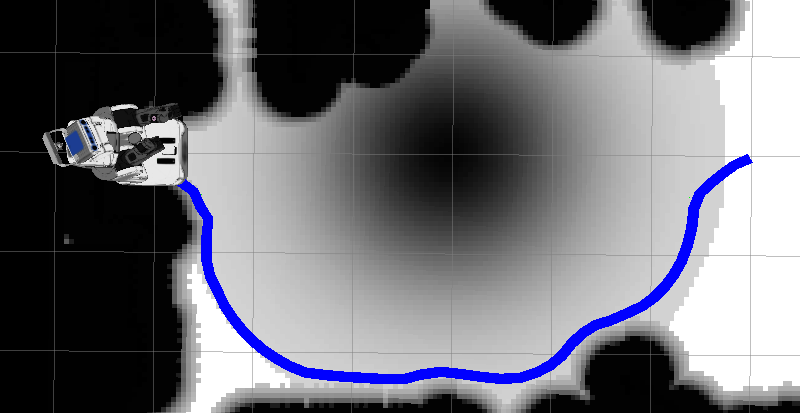
\includegraphics[width=\rrrr\textwidth]{graphix/250-p9.png}
\label{fig:d4}}
\subfloat[$A=250$, $\sigma=1.20$]{
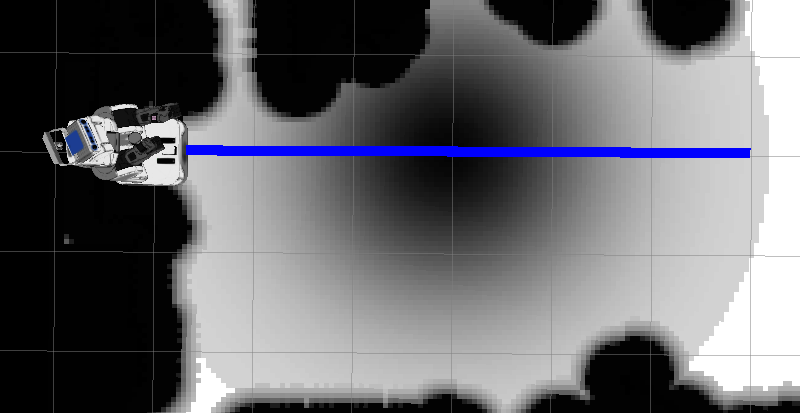
\includegraphics[width=\rrrr\textwidth]{graphix/250-1p2.png}
\label{fig:d5}}
\subfloat[$A=150$, $\sigma=1.20$]{
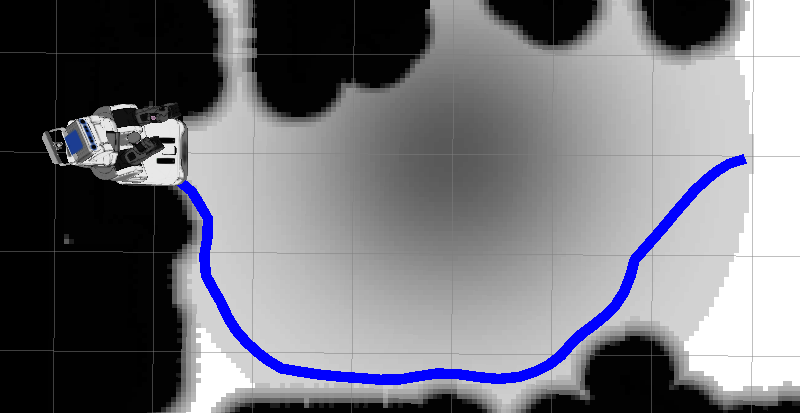
\includegraphics[width=\rrrr\textwidth]{graphix/150-1p2.png}
\label{fig:d6}}
\caption{Real plans generated by the ROS Navigation Stack - As the variance increases (a)-(d), the path gets further from the obstacle. However, in (e) when the variance is over 1, the path reverts to straight through. However, by setting the amplitude to a smaller number, while keeping the variance constant, (f), we can again derive a not straight plot.  }
\label{fig:realdata}
\end{figure*}


\section{Discussion}
\subsection{Practical Parameter Tuning}
\subsection{Future Work}
Metrics, discrete, 8-connected

Different angles

Discussion of interaction of lethal and nonlethal (can go near a person if you have to) (you shall not pass)

optimally suboptimal

square plans are dumb



\bibliographystyle{plainnat}
\bibliography{nonlethal}

\end{document}


